\documentclass[letterpaper,10pt]{article}
\usepackage[top=2cm, bottom=1.5cm, left=1cm, right=1cm]{geometry}
\usepackage{amsmath, amssymb, amsthm,graphicx}
\usepackage{fancyhdr}
\pagestyle{fancy}

\lhead{\today}
\chead{Stat 740 Assignment 5}
\rhead{Justin Hood}

\newcommand{\Z}{\mathbb{Z}}
\newcommand{\Q}{\mathbb{Q}}
\newcommand{\R}{\mathbb{R}}
\newcommand{\C}{\mathbb{C}}
\newtheorem{lem}{Lemma}

\begin{document}
\begin{enumerate}
\item We consider the data contained in the FuelEconomy.csv file. This data is a sample of cars and associated MPG values obtained from testing.
\begin{enumerate}
\item To begin, we consider plotting the data.
\begin{center}
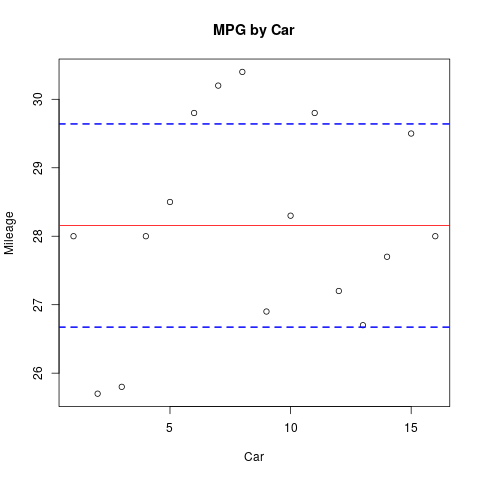
\includegraphics[scale=.7]{1a.png}
\end{center}
Here, we have superimposed the mean and bars corresponding to one standard deviation from the sample in red and blue respectively.
\item Next, we consider how we might construct a 95\% confidence interval for the mean fuel economy using a $t$ distribtution. Setting $\alpha=1-.95=0.05$, we compute the ``critical" $t$-value to be, $t^*_{.025,16-1}=2.13145$. Hence, we construct our interval in $R$ as,
\[I=\left[\bar{x}\pm t^*\frac{s}{\sqrt{n}}\right]=\left[28.15625\pm 2.13145\frac{1.48412}{\sqrt{16}}\right]=\left[27.36542,\ 28.94708\right]\]
\item Finally, we consider constructing a 95\% confidence interval using a bootstrap. To perform this operation, we will construct 100 samples of size $n=16$ from the original data by sampling with repetition. Then, from these new samples, we will extract the means, and look at the quantiled data to determine a confidence interval. A pictographic display of the first 100 samples follows,
\begin{center}
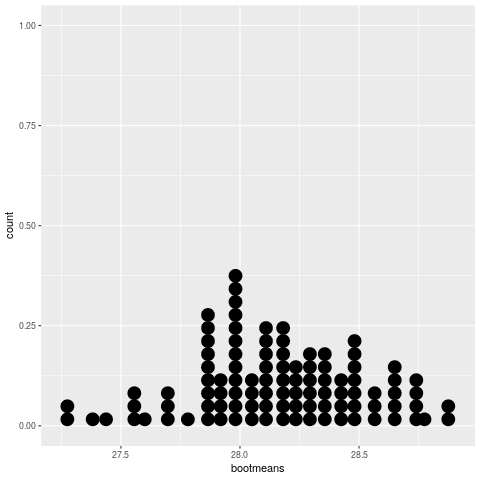
\includegraphics[scale=.65]{econdot.png}
\end{center}
We show the first 100 samples for the visual ease. After performing the full 1000 sample process, we find the histogram of the new sample mean data,
\begin{center}
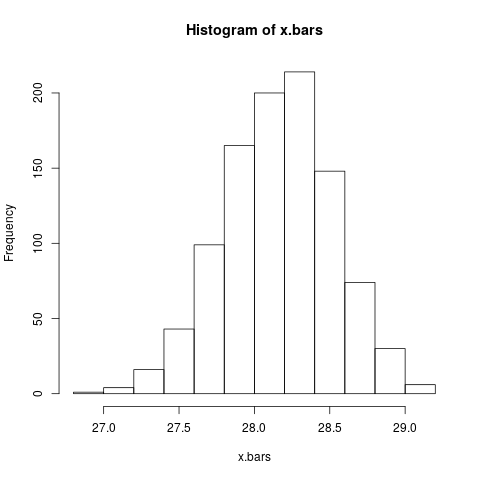
\includegraphics[scale=.65]{econhist.png}
\end{center}
We see that our data falls into a nice bell curve, as desired, and that the data appears to have a peak around $\approx 28.2$, aligning with our original data mean. Finally, we extract the lower and upper 2.5\% quantile data to construct our interval, which becomes,
\[I=\left[27.46187,\ 28.83156\right]\]
We note that this new interval is slightly smaller than the one produced by the $t$ distribution. 
\end{enumerate}
\item We consider the eye color data from EG12-15EYES.csv.
\begin{enumerate}
\item First, let us construct a visual representation of the data,
\begin{center}
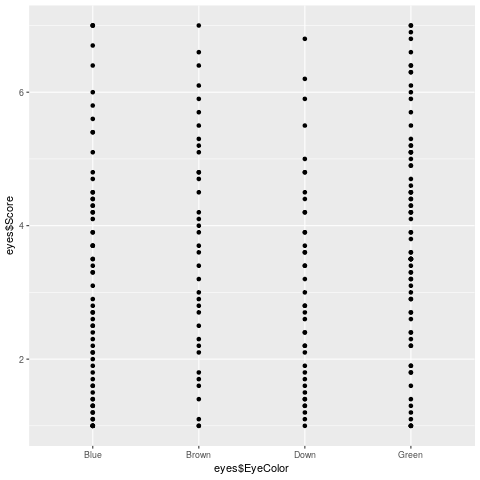
\includegraphics[scale=.6]{2qplot.png}
\end{center}
We see that this plot is quite cluttered due to the high volume of data, so we consider an alternative plot,
\begin{center}
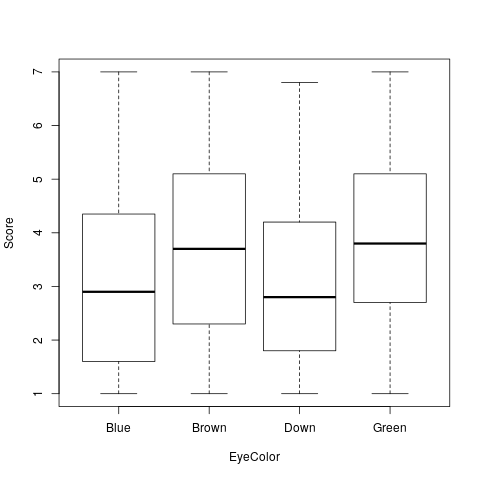
\includegraphics[scale=.6]{2stem.png}
\end{center}
From this second plot, we see that visually, there appear to be differences between the factor levels, as there are two groupings of level means.
\item Next, we compute a one way ANOVA analysis to compare the means of the different levels. Using $R$, we obtain the following ANOVA table,
\begin{center}
\begin{tabular}{|l|c|c|c|c|c|}
\hline
& Df & SS & MSQ & F-Val & Pr($>$F)\\\hline
Eye Color & 3 & 24.42 & 8.1399 & 2.8941 & 0.03618\\\hline
Residuals & 218 & 613.14 & 2.8126 &&\\\hline
\end{tabular}
\end{center}
Based on our ANOVA test, we see that the $p$ value is $p=0.03618<0.05$. Thus, we reject the null hypothesis, that the factor means are equal, in favor of the alternative, that at least one mean is different.
\item To construct 95\% confidence intervals on the data, we consider the pairwise possibilites for differences between the factor levels. We have, $\binom{4}{2}=6$ different pairwise differences to consider,
\begin{enumerate}
\item Brown-Blue
\item Down-Blue
\item Green-Blue
\item Down-Brown
\item Green-Brown
\item Green-Down
\end{enumerate}
Note, the order does not matter, as we are looking for spread about zero. Based on this, we consider Tukey's method for comparisons. Using $R$ we may easily obtain the numerical data corresponding to each of the aforementioned intervals, but a graphical expression is also obtained,
\begin{center}
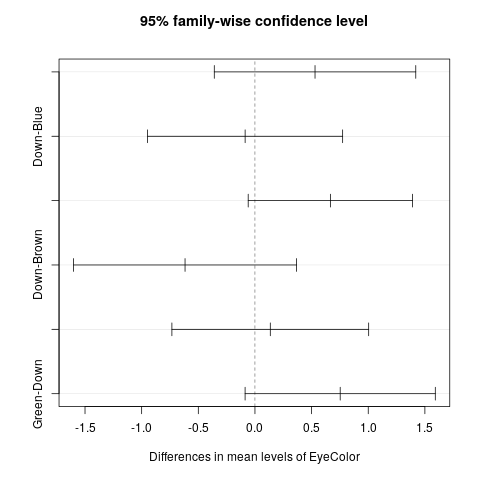
\includegraphics[scale=.65]{tukey.png}
\end{center}
Under ANOVA's assumed null hypothesis, these intervals shold all be centered about zero. And indeed, we see that some of the differences are, but there are also a number of them that are not, further confirming our existing results of rejection of the null with ANOVA.
\item We now consider the results from $(a)$ and $(b)$. In $(a)$, we concluded graphically that we did not think that the means were all equal. In $(b)$ we concluded numerically that this was the case, and we also conisdered the pairwise differences. Based on the plot in $(a)$, we would think that Brown and Green eyes induce a higher attitude towards the brand than Blue and Downward facing. Consider now, the CI's computed in $(c)$. First, consider the <1st, 4th, 5th> intervals. These correspond to
Brown-Blue, Down-Brown, Green-Brown. We see that the 1st interval has a positive center, the 4th a negative center, and the 5th an approximately zero center. This makes sense from our assertion that Brown has a higher attitude. Similarly, we see the same effects with Green eyes. From this, we might conclude that Brown and Green eyes are better for advertising based on this test.
\item If we were to use Bonferroni simultaneous CI's, we would have different widths than the above. These intervals would each be constructed using $\alpha=0.05/6=.008333$. As such, we would expect their widths to be wider, and consequently more conservative.
\end{enumerate}
\item We consider the data within the file PremiumDistribution.txt.
\begin{enumerate}
\item First, let us again construct boxplots of the data partitioned by ``agent".
\begin{center}
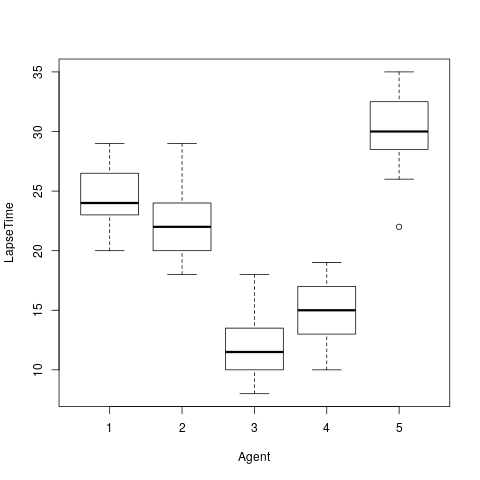
\includegraphics[scale=.65]{3box.png}
\end{center}
Here, we see that there appears to be a fairly large difference in the lag times based on the agent. This being said, we note that the boxes for each agent are all approximately the same width for the IQR. From this, we infer that the variances are all approximately similar.
\item Next, we compute the ANOVA table for the data using $R$,
\begin{center}
\begin{tabular}{|l|c|c|c|c|c|}
\hline
& Df & SS & MSQ & F-Val & Pr($>$F)\\\hline
Agent & 4 & 4430.1 & 1107.53 & 147.23 & $2.2e-16$\\\hline
Residuals & 95 & 714.6 & 7.52 &&\\\hline
\end{tabular}
\end{center}
\item Here, we are testing whether the mean lapse time differs for the different agents. Let, $\mu_i$ be the mean lapse time for a given agent. Our hypothesis then becomes,
\begin{align*}
H_0: & \mu_1=\mu_2=\mu_3=\mu_4=\mu_5\\
H_A: & \mu_i\neq \mu_j \text{ for at least one pair i,j in [1,5]}
\end{align*}
Our ANOVA test statistic computed before is the relevant test statistic for testing the above hypotheses, that there is some difference in the means of the different agents. Using the $F$ statistic, we obtain the $p$ value of $p=2.2e-16$. Given that we are testing this lapse with an $\alpha=0.10$, we see that we will clearly reject the null hypothesis, and conclude that there is some difference in lapse time depending upon which agent you look at.
\item Given that we have rejected the null hypothesis, it is necessary to look at the simultaneous condfidence intervals. For this problem, we consider both the Bonferroni simultaneous interval and the Tukey interval. For our 95\% interval, using Tukey's method in $R$, we obtain the following plot,
\begin{center}
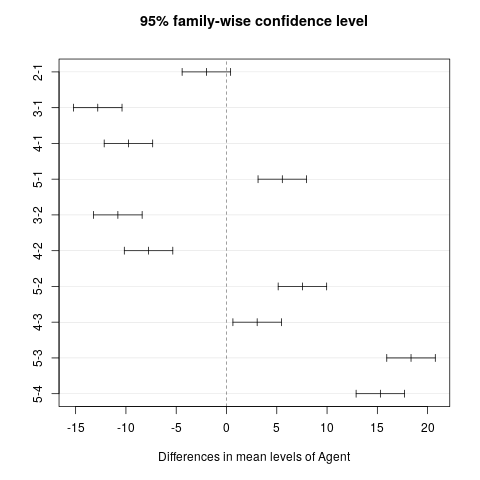
\includegraphics[scale=.65]{3tukey.png}
\end{center}
Here, we may graphically compare the different methods about zero. We see that zero clearly falls into the interval between Agent 2 and Agent 1, and so we see that there is probably no significant difference between the two agent's lapse times. We also see that the interval between Agent 3 and Agent 4 does not quite contain zero, but is very close, so there is a potential for a lack of difference between them. Other than these two pairs, we see that there appears to be a non-zero difference between the rest. To further conferm, we compute the Bonferroni intervals in $R$ to the same results. Again, Agents 1 and 2 contain zero in their difference interval, and Agents 3 and 4 are very close to having zero in their difference interval.
\item Based on the results of this confidence testing, as well as the original data, we conclude that Agent 5 has the longest lapse time of all the agents. The difference between Agent 5 and the rest never contain the zero, and its mean is the greatest of the original data. Conversely, we conclude that agents 3 and 4 have the slowest lapse time. Because we cannot definitively state that there is a difference between them, and they share the lowest original means, we conclude that they are the lowest pair.
\end{enumerate}
\item Let us not consider the value of $R^2$ within our ANOVA model. Using the ANOVA table, we may compute this as,
\[R^2=1-\frac{SSE}{SSTO}\]
From our data in problem 3, we see that our $R^2$ value is,
\[R^2=1-\frac{714.6}{5144.7}=0.8610998\]
In keeping with this idea, we shall now construct a bootstrap 95\% confidence interval to analyze $R^2$, using the soft drink data from before. As in question 1, we begin by selecting 1000 strap samples, of size $n=100$ from the soft drink data, each time sampling with replacement. From each of these 1000 samples, we compute the ANOVA model and compute $R^2$ as above. This data is recorded each time, and the overall results analyzed. After the first 100 samples, we create a dot plot to get a sense of what these $R^2$ values are doing. The plot follows,
\begin{center}
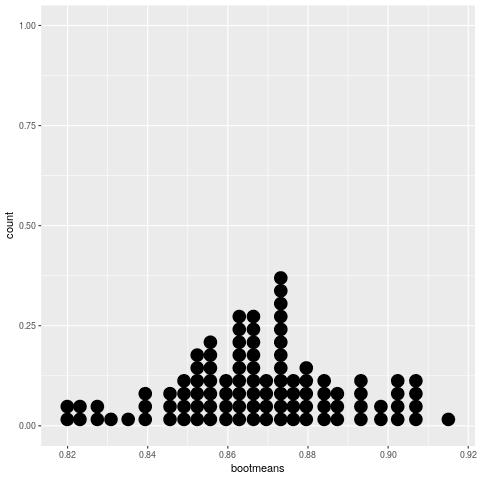
\includegraphics[scale=.65]{R2dot.png}
\end{center}
We see a peak forming between $0.86$ and $0.88$, which falls in line with our original model $R^2$ value. Once the 1000 samples have been computed, we may now construct a histogram of the results,
\begin{center}
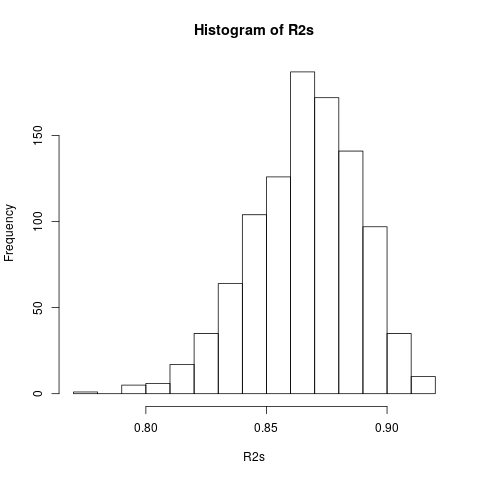
\includegraphics[scale=.65]{R2hist.png}
\end{center}
Again, our peak falls where we would expect it to, and it has a nice bell curve to the overall shape. Finally, using $R$, we compute the 95\% interval from this data,
\[I=(0.8190444,\ 0.9038352)\]
So, we see that our bootstrapped estimate of $R^2$ says that it can account for between 81.9\% and 90.4\% of the variance in the data. This is good, as higher values of $R^2$ imply that our model constructed with ANOVA accounts for the variance in the data. Since $r$ values are always higher than their corresponding $R^2$ values, we see that our ``correlation coefficient" seems to be above $\sqrt{0.8190444}=0.90501$, or 90\%. Thus, we are condfident in our model that we have constructed.
\item We shall now consider the innate ``Orchard Sprays" data set in $R$. To begin, we look at the head of the data frame:
\begin{center}
\begin{tabular}{rrrrr}
& decrease & rowpos & colpos & treatment\\
1 & 57 & 1 & 1 & D\\
2 & 95 & 2 & 1 & E\\
3 & 8 & 3 & 1 & B\\
4 & 69 & 4 & 1 & H\\
5 & 92 & 5 & 1 & G\\
6 & 90 & 6 & 1 & F
\end{tabular}
\end{center}
So, we see that we have four columns of data, with the two most relevant being the decrease and treatment columns. Given that we are working with an 8x8 latin square design, we know that there are 8 different treatments of the sulphur solution.
\begin{enumerate}
\item To begin, we consider a box plot of the data.
\begin{center}
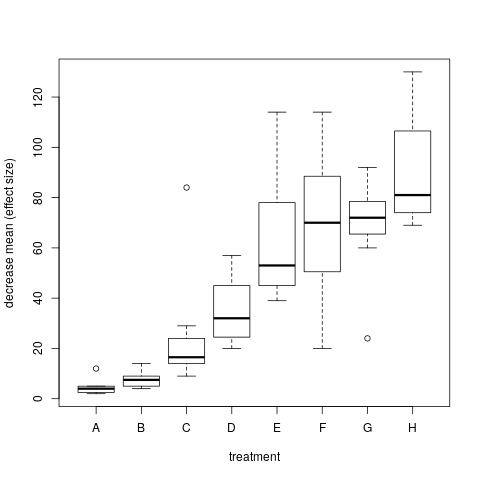
\includegraphics[scale=.65]{5box.png}
\end{center}
From this view of the data, we see that the means for a given treatment seem to vary a great deal, as well as each treatment having different IQR ranges. As such, we next look at the standard deviations for each treatment,
\begin{center}
\begin{tabular}{r|r}
Treatment & Standard Deviation \\\hline
A & 3.204350\\ B & 3.292307\\ C & 24.429198\\ D & 13.437687\\ E & 26.909571\\ F & 29.189039\\ G & 20.142351\\H & 24.223660
\end{tabular}
\end{center}
Here we see that the deviations for some treatments are much larger than others. The deviation for treatment $F$ is 9.11 times larger than $A$. This result is in violation of our ANOVA assumptions, and as such, we must consider an alternative model. The model we shall use is the Kruskal-Wallis Test. Our hypotheses are the same as under the ANOVA model,
\[H_0: \mu_A=\mu_B=\ldots=\mu_H,\ \ H_A:\exists i,j\in[A,B,C,D,E,F,G,H]\text{ s.t. } \mu_i\neq \mu_j\]
Using $R$, we shall sort the data by rank and then compute our corresponding test statistic. Here, our test statistic is,
\[H=-3(n+1)+\frac{12}{n(n+1)}\sum_i\frac{R_i^2}{n_i}\sim \chi^2_{g-1}\]
From $R$'s built in function for the Kruskal test, we obtain the following results:
\[H=48.874,\ H^*=7.814728,\ \ p=2.402e-8\]
Here, we see that our test statistic is greater than the critical value, and as such $p<\alpha$. So, we reject our null hypothesis, that the means are equal in favor of the alternative, that there is at least one mean that is significantly different than the others.
\item Based on our initial box plot, we noted that as the concentration of Sulphur decreases, the decrease mean increases. So, when we consider the most effective concentrations, we shall start with treatment A. Using a Bonferroni interval, we compute the interval for the difference between treatments A and B.
\[I=(-9.246204,\  3.246204)\]
Here, we see that 0 is within the interval, so we consider also the differences between A and C/D. These intervals are,
\begin{align*}
I_{AC} &= (-62.45651,\ 21.20651)\\
I_{AD} &= (-53.037125,\  -7.712875)
\end{align*}
Here, we see that we may finally note a significant difference between A and D. So, the most effective treatment appears to be A, but since we cannot definitively find a difference between A and B or A and C, we see that treatments $A,B,C$ are the most effective.
\end{enumerate}
\end{enumerate}
\end{document}
